\chapter{Háttérismeretek}

A célja ennek a fejezetnek, hogy összefoglaljam a témám értelmezéséhez szükséges alapismereteket, fogalmakat és bemutassam a használt technikai eszközöket. Ebben a fejezetben leírtak lesznek szükségesek ahhoz, hogy a későbbi fejezeteket teljességükben lehessen értelmezni.

Az első fejezet tartalmazza a későbbiekben használt szakszavakat az elterjedt szakirodalmakban található leírások alapján. 

Ezután következik az autóipari kiberbiztonság szabályozási környezete, azon belül is elsősorban az ISO/SAE 21434 szabvány, ami lefedi a terület alapvető irányelveit, valamint ad egy kezdetleges metodológiát a kiberbiztonsági kockázatelemzésre.

Ezt követi egy leírás az IT biztonság területén már ismert fenyegetésmodellezés technikákról és keretrendszerekről.

Végül pedig a munkám során alkalmazott eszközök és technológiák rövid ismertetése olvasható.

\section{Kiberbiztonsághoz kapcsolódó alapfogalmak}

Ebben a fejezetben található minden továbbiakban nem általánosnak vehető, az autóipari és a kiberbiztonsági területeken használt szakszavaknak a definíciói. Ezek a leírások elsősorban a már elérhető kutatásoknak, szabályozásoknak és szabványoknak a szójegyzékére építenek.

\begin{itemize}
    \item \textbf{Termék (product / item):} Egy önmagában is értelmezhető és értékesíthető rendszer, amelynek a biztonságát biztosítani kell. Ez lehet egy komponens vagy komponensek csoportja és egy jármű-szintű funkcionalitást valósít meg, pl. kormányrendszer, fékrendszer, szoftver-frissítési infrastruktúra
    \item \textbf{Komponens (component):} Logikailag és/vagy technikailag szeparálható elem    
    \item \textbf{Úthasználó (road user):} Személy aki valamilyen formában az utat használja, pl. gyalogos, autóvezető, utas, stb.
    \item \textbf{Kiberbiztonsági terv (cybersecurity concept):} Kiberbiztonsági követelményei egy terméknek, az üzemeltetési környezetnek, támogató információk a mitigációkhoz
    \item \textbf{Kiberbiztonsági specifikáció (cybersecurity specification):} Részletesebb kiberbiztonsági követelmények allokálva az architektúrális tervre
    \item \textbf{Kiberbiztonsági cél (cybersecurity goal):} Magas-szintű kiberbiztonsági követelmény
    \item \textbf{Kiberbiztonsági állítás (cybersecurity claim):} Állítás egy kockázatról
    \item \textbf{Mitigáció (mitigation / cybersecurity control):} Kockázatmódosító intézkedés
    \item \textbf{Érték (asset):} Egy tárgy ami értékkel rendelkezik
    \item \textbf{Kiberbiztonsági tulajdonság (cybersecurity property):} Egy attribútum amelyet meg kell védeni, pl. sértetlenség, bizalmasság, elérhetőség
    \item \textbf{Károkozás (damage scenario):} Egy kedvezőtlen következmény amely hatással van az úthasználóra
    \item \textbf{Fenyegetés (threat scenario):} Egy lehetséges kompromittálása valamilyen érték kiberbiztonsági tulajdonságának, amely egy károkozáshoz vezethet (pl: egy szoftveres sérülékenység kihasználása)
    \item \textbf{Támadási útvonal (attack path):} Események (pl: egy fenyegetés megvalósulása) egymás utáni bekövetkezése, amely egy károkozást realizálnak
    \item \textbf{Támadási lépés (attack step):} Az egyes események amelyeknek az egymás utáni sorozata egy támadási útvonalat realizál
\end{itemize}

\section{Autóipari kiberbiztonsági szabályozások és szabványok}

Az autóipari kiberbiztonság területe ellentétben az üzembiztonsággal vagy a bővebb IT biztonsággal még csak pár éves múltra tekint vissza, emiatt az itt alkalmazandó szabályozások és szabványok még csak az első változatukban kerültek kiadásra. 

\subsection{UN ECE R155}
Az első specifikusan autóipari szabályozás az Egyesült Nemzetek által kiadott 155-ös számú szabályozás a kiberbiztonságról és a kiberbiztonság kezelő rendszerekről és járművek engedélyeztetésének kapcsolatáról (UN ECE R155\cite{R155}). Ennek a szabályozásnak kell megfelelnie a járműgyártóknak és beszállítóiknak az összes 2024 után megjelenő járműmodell engedélyeztetéséhez.

Ez a szabályozás már tartalmazza az igényt a kockázat-alapú kiberbiztonsági kezelés szükségességére. Ami annyit tesz, hogy a biztonsági szolgáltatásokat az alapján kell meghatározni, hogy egy kiberbiztonsági fenyegetés esetleges bekövetkezése mekkora hatással lenne a védendő autóipari termékre.

Szintén már megtalálhatjuk az autóipari termékek életciklusának különválasztását fejlesztési, gyártási és gyártás utáni fázisokra, ami mutatja azt, hogy a kiberbiztonsági szempontból fontos figyelembe, venni, hogy az életciklus különböző szakaszain más-más fenyegetésekre lehet számítani, és ennek megfelelően más követelmények is lesznek érvényesek a termékre.

A dokumentum a továbbiakban követelményeket határoz meg, hogy milyen folyamatokon kell keresztülmennie egy autóipari terméknek, ahhoz, hogy az a közúti használatra engedélyt kapjon. 

\subsection{ISO/SAE 21434}

A másik, már technikaibb szintű, szintén 2021-es megjelenésű, irányadó szabvány az autóipari kiberbiztonsági mérnökségről szóló ISO/SAE 21434 "Road vehicles - Cybersecurity engineering"\cite{ISO21434}. Ezt a szabványt közösen fejlesztette és adta ki 2021 augusztusában az International Standards Organization (ISO) és a Society of Automotive Engineers (SAE).

Ez a szabvány kezdett el követelményeket megfogalmazni az autóipari rendszerek (E/E) kiberbiztonsági kockázatkezelésének menetére, valamint a biztonság fejlesztésére és kezelésére. A felépítése emlékezetheti az olvasóját a már jóval ismertebb ISO 26262 "Road vehicles - Functional safety" szabványra, amely ugyanazon termékek üzembiztonságának a kezelésére és elemzésére fókuszál.

A szabvány először a tervezési, fejlesztési, gyártási, üzemeltetési, karbantartási és kivezetési fázisokra fogalmaz meg követelményeket, valamint tartalmaz egy fenyegetés elemző és kockázat értékelő eljárást amelynek a Threat Analysis and Risk Assessment (TARA) nevet adták.

Továbbá tartalmaz más követelményeket a kiberbiztonsági elvárások kezelésére különböző menedzsment és organizációs szintekre, azonban ezek ismerete nem tartozik a témám látókörébe.

Dolgozatom kifejezetten a tervezési fázishoz tartozó kockázatelemzés végrehajtására vonatkozó követelményeket veszi alapul. A későbbi bemutatásuk során felfedezhető lesz, hogy a kockázatelemzés iteratív használatának szükségessége az életciklus különböző fázisaiban, azonban a termék üzemeltetési környezetére vonatkozó védelmet ebben a tervezési fázisban határozzuk meg. Ezzel elkerülve a magasabb költségű utólagos fejlesztéseket.

\subsubsection{Követelmények a tervezési fázisra}
A tervezési fázis egy autóipari termék életciklusában a kiindulópont. Az ebben a fázisban végzett kiberbiztonsági tevékenységek célja, hogy (i) definiálásra kerüljön az elemzendő termék, a környezete és interakciói, (ii) meghatározzák a kiberbiztonsági célokat és állításokat valamint, hogy (iii) elkészüljön a kiberbiztonsági terv.

A \textbf{termék definíciója} tartalmazza a termék határait, feladatait, valamint az előzetes architektúrát. Célunk itt az, hogy összegyűjtsük az elemzéshez szükséges információkat.

A \textbf{kiberbiztonsági célok és állítások} meghatározásához szükséges a TARA elvégzése, aminek az eredményeképp születnek meg, az egyes kockázatok kezelésére vonatkozó döntések, amelyek alapján eldönthetjük, hogy a kockázathoz egy célt vagy állítást kell megfogalmaznunk. A cél fogja meghatározni a magas-szintű követelményt amit a termék fejlesztése során figyelembe kell venni, míg az állítás azt határozza meg, hogy az adott kockázat mitigálása valamilyen okból már teljesült vagy a teljesülése szükségtelen.

Ezután készülhet el a \textbf{kiberbiztonsági terv}, amelyben az egyes mitigációkat határozzuk meg a célok elérésére, a célokat tovább finomítjuk követelményekké, majd azokat allokálhatjuk a termékre vagy egyes komponensekre.

\subsubsection{Követelmények a fenyegetéselemzésre és kockázatértékelésre}
A TARA bemenete a termék definíció, és ez alapján lehet elvégezni a hét lépésből álló kockázatelemzési eljárást aminek a kimenete az egyes fenyegetések kockázati értékkel, valamint az azok kezeléséről szóló döntés.

Az első lépése a kockázatelemzésnek az \textbf{érték azonosítás}. Ennek a lépésnek két célja van. Az egyik, hogy a lehetséges \textit{károkozásokat} azonosítsuk és azok segítségével az egyes \textit{értékeket} is meghatározzuk, a másik pedig, hogy az értékekhez \textit{kiberbiztonsági tulajdonságokat} rendeljünk. 
A károkozások tartalmazhatják a kár körülírását, a releváns értékeket és a kapcsolatot a járműfunkcionalitás és a kedvezőtlen következmény között.
Az értékek azonosítására használhatjuk továbbá a termékleírást, a \textit{fenyegetések} definiálását vagy már létező katalógusokat.

A kockázatelemzés második lépése a \textbf{hatásértékelés}. Itt a célunk az egyes lehetséges károkozásokat és azok következményeit valamilyen keretrendszer mentén értékelni. Egy lehetőség, amit több szabvány is említ, az az SFOP alapú értékelés. Az SFOP négy dimenziót határoz meg amiben el kell végezni az értékelést. Ezek az üzembiztonsági hatás (safety), gazdasági hatás (financial), üzemeltetési hatás (operational), valamint az adatvédelmi hatás (privacy).

A kockázatelemzés harmadik lépése a \textbf{fenyegetések azonosítása}, amelyekhez hozzá kell rendelni a támadott \textit{értéket}, annak a kompromittált \textit{kiberbiztonsági tulajdonságát}, valamint a kompromittálás okát. A szabvány szerint ezek azonosítására lehet egyrészről csoportos, brainstorming alapú vagy szisztematikus, keretrendszerek által meghatározott módszereket is alkalmazni. Az utóbbi esetben javasolt valamilyen ismert fenyegetésmodellezési megközelítést használata. Néhány felsorolt példa ezekre az EVITA, TVRA, PASTA és a STRIDE.

A negyedik lépés a \textbf{támadási útvonal elemzés}. Az elemzés során a szabvány szerint top-down vagy bottom-up megközelítést is használhatunk. Előbbi esetben támadási fákat, támadási gráfokat, utóbbi esetben már ismert sérülékenységekre alapulót.

Az ötödik lépés a \textbf{támadás megvalósíthatóságának vizsgálata}, ahol több már létező keretrendszert alkalmazhatunk az egyes támadási útvonalak kiértékelésére. 

A hatodik lépés a \textbf{kockázatiérték meghatározás}. Itt egy egytől ötig terjedő skálán értékeljük a fenyegetési szcenáriókat a hatásértékek és a megvalósíthatósági értékek alapján.

A hetedik és egyben utolsó lépés pedig a \textbf{kockázatkezelési döntés}, amikor az egyes kockázatok kezeléséről hozhatunk döntést. A kockázatokat elkerülhetjük, csökkenthetjük, megoszthatjuk, valamint megőrizhetjük.

Jól látható, hogy ezek a követelmények elég általánosak, sok döntési jogosultságot helyez a folyamatot bevezető személyekre, emellett viszont magas szinten jól körülírt követhető lépéseket határoz meg amelyek megfelelnek más szabályozások feltételeinek és képes eljuttatni a mérnököt a konkrét megvalósítandó intézkedések meghatározásához. 

\section{Fenyegetésmodellezési keretrendszerek és módszerek}

A fenyegetésmodellezés egy olyan folyamat, aminek segítségével azonosítani tudjuk a lehetséges fenyegetéseket, valamint segítenek azok értékelésében.

Ez a folyamat már viszonylag régóta elterjedt a kiberbiztonsági szakmában és támogató jellegű kapcsolatban áll a kockázatelemzésekkel. Amíg a fenyegetésmodellezés célja a fenyegetések meghatározása, a kockázatelemzés az ami segít nekünk a feltárt fenyegetések kezelésének priorizálásában vagy esetenként az egyes fenyegetések elhagyásában.

Tágabb értelemben akár a kockázatelemzést is vehetjük a fenyegetésmodellezés részének, azonban az ISO/SAE 21434 szabványban leírt folyamat is különválasztja azokat és a fenyegetésmodellezést kifejezetten a fenyegetések meghatározására javasolja.

\subsection{CIA és AAA}

Bár még nem is egy teljes fenyegetésmodellezési keretrendszer a CIA háromszög vagy CIA triád, mégis a legtöbb kiberbiztonsági elemzés az ezen betűszó által kifejezett modellt alkalmazza.

Már korábban beszéltünk kiberbiztonsági tulajdonságokról, itt a CIA által definiáltak használjuk, ezek a bizalmasság (confidentiality), sértetlenség (integrity) és elérhetőség (availability). 

Szintén előfordul ennek a modellnek a bővítése egyéb tulajdonságokkal, ilyenek a szoftverbiztonság esetén használt AAA modell elemei amelyek az egyediség (authenticity), engedélyezhetőség (authorizability), valamint az elszámoltathatóság (accountability).

Adott értéknek a tulajdonságait meghatározhatjuk az alábbi kérdések megválaszolásával:
\begin{itemize}
    \item \textbf{Bizalmasság}: Harmadik fél szerezhet-e tudomást az értékről, annak tartalmáról?
    \item \textbf{Sértetlenség}: Az érték módosulása vezethet-e nem várt következményekhez?
    \item \textbf{Elérhetőség}: Az érték hiánya vezethet-e nem várt következményekhez?
    \item \textbf{Egyediség}: Kell-e az érték eredetét biztosítani felhasználása előtt?
    \item \textbf{Engedélyezhetőség}: Szükséges-e az adott értékhez való hozzáférés korlátozása?
    \item \textbf{Elszámoltathatóság}: Szükséges-e az adott értékhez való hozzáférések, módosulások visszakövethetősége?
\end{itemize}

A továbbiakban ezeket a modelleket fogom alkalmazni a kiberbiztonsági tulajdonságokként, azonban ezek módosíthatók, elhagyhatóak, cserélhetőek és bővíthetőek felhasználási környezetüktől függően. Az én esetemben a CIA elegendő lesz, hiszen autóipari beágyazott rendszerekben a szoftver szinten azon tulajdonságok relevánsabbak. Az üzenet egyediségének hamisítása már az eredeti üzenet egyfajta sérülését vonja magával, ez a sértetlenség tulajdonság által már kezelve van. Az engedélyezhetőség pedig már bonyolultabb operációs rendszerek használatánál kerül elő, ami külön felhasználókat és hozzáféréseket tud definiálni. Ez bizonyos formában az autóiparban is fellelhető, de nem abban a komplexitásban mint Linux vagy Windows alapú rendszereknél. Az elszámoltathatóság szintén problémás mivel ennek a biztosítása, a beágyazott rendszerek limitált hardvererőforrásai miatt nem tud azzal a granularitással létezni, ahogy a hozzáférések számon lennének tartva IT rendszereknél.

\subsection{STRIDE}
A STRIDE egy modell, amely számítógépes kiberbiztonsági fenyegetések azonosítására lett kifejlesztve a Microsoft által 1999-ben. A nevét a hat fenyegetéstípusról kapta, ezek és a jelentésük:

\begin{itemize}
    \item \textbf{Spoofing:} Megszemélyesítés, amikor a rendszer hamisan érzékeli az információ küldőjének a kilétét
    \item \textbf{Tampering:} Valamilyen információ megváltoztatása
    \item \textbf{Repudiation:} Annak az állítása, hogy valamit nem te csináltál vagy nem is történt meg
    \item \textbf{Information disclosure:} Egy támadó képes hozzáférni olyan információhoz amire nincs jogosultsága
    \item \textbf{Denial of Service:} Erőforrások túlterhelése miatt szolgáltatás elérhetetlenné tétele
    \item \textbf{Elevation of privilige:} Egy támadó képes olyan művelet elvégzésére, amire nincs felhatalmazva
\end{itemize}

Ez első ránézésre egy jó lehetséges kategorizálást ad meg nekünk fenyegetésekhez, valamint kibővíthető ezek kapcsolata az azonosított értékekhez és kiberbiztonsági tulajdonságaikhoz. Tehát az egyes fenyegetés típusok egy bizonyos tulajdonság sérülését célozzák.

\begin{table}[h]
    \centering
    \begin{tabular}{rl}
        Spoofing & Egyediség (authenticity) \\
        Tampering & Sértetlenség (integrity) \\
        Repudiation & Letagadhatatlanság (non-repudiability) \\
        Information disclosure & Bizalmasság (confidentiality) \\
        Denial of Service & Elérhetőség (availability) \\
        Elevation of privilige & Engedélyezhetőség (authorizatiability) \\
    \end{tabular}
    \caption{Fenyegetések kapcsolata kiberbiztonsági tulajdonságokkal}
    \label{tab:my_label}
\end{table}

Ebből jól látható, hogy az egyes értékekhez a tulajdonságaik alapján már azonosíthatjuk az azok kompromittálását célzó lehetséges fenyegetéseket.

Ezekből én mivel csak a CIA tulajdonságait használom, az én esetemben a Tampering, Disclosure és Denial fenyegetések lesznek a tulajdonságokból származtatva.

\section{Autóipari rendszerek általános tervezése és modellezése}

A diplomamunkám sajátossága abból adódik, hogy amíg az általános IT rendszereknek vagy azok egyes elemeinek az architektúrális tervezése kevésbé jellemző, addig a kiber-fizikai rendszereknél, azon belül is a járműveknél, a rendszer komplexitása és az üzembiztonság kritikussága miatt, nagy hagyománya van ezeknek az átfogó dokumentálására már a tervezés kezdeti szakaszában.

\subsection{V-modell}

A V-modell egy szoftverfejlesztési folyamat amelyet az ASPICE szabvány adaptál az autóiparban. Lényegében arról szól, hogy a fejlesztés V alakban történik, ahol bal oldalt fentről lefele történik a tervezés és a fejlesztés, a jobb oldalon pedig minden lépéshez tartozik egy verifikációs vagy validációs lépés.

Nemrégiben kapott az ASPICE\cite{ASPICE} szabvány egy kiegészítést a kiberbiztonsági mérnöki folyamatokhoz amelyeket részben az ISO 21434 is definiált. Ezekről egy összefoglaló a \ref{fig:ASPICE} ábrán látható.

\begin{figure}[!ht]
\centering
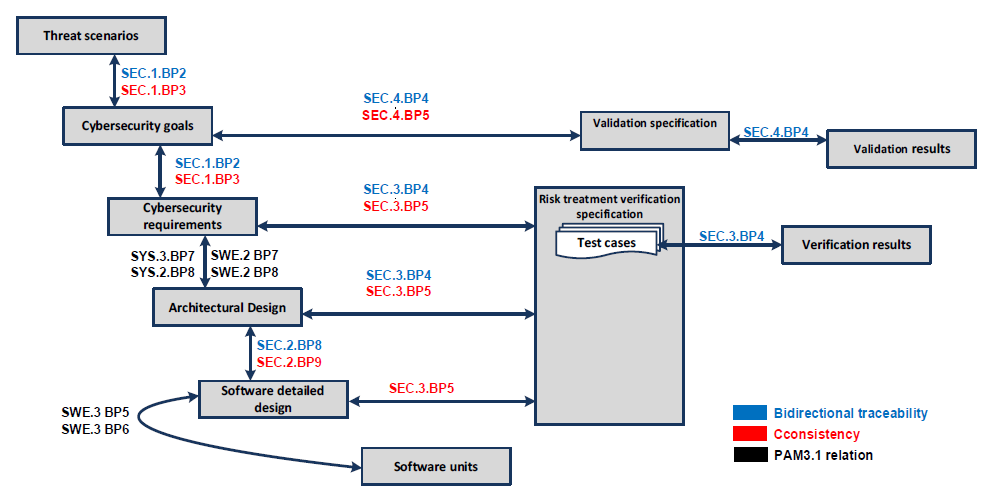
\includegraphics[width=150mm, keepaspectratio]{figures/02_ASPICE.png}
\caption{Az ASPICE javaslata kiberbiztonsági folyamatokra\cite{ASPICE}}
\label{fig:ASPICE}
\end{figure}

Szintén érdemes itt megjegyezni, hogy az általam javasolt metodológia egyfajta visszacsatolást (feedback) tenne lehetővé az \textit{Architectural design} és a \textit{Threat scenarios} lépések közt. De erről később bővebben lesz szó.

\subsection{UML és SysML}

A komplex E/E architektúrák esetén, mint amilyenek az autóipari beágyazott rendszerek, jellemző valamilyen formában a rendszermodellek jelenléte és karbantartása a termék életciklusa alatt. Erre elsősorban a SysML (System Modeling Language) van használva, ami egy bővítése az UML-nek (Unified Modeling Language).\\

% UML
Az UML egy általános felhasználású grafikus modellezési nyelv, amelynek célja a rendszerek specifikálása, a felépítésük leírása, vizualizálása és dokumentálása a fejlesztésben érdekelt minden résztvevő számára.

Az UML több diagram típust különböztet meg, azokat elsősorban két kategóriába sorolhatjuk, az egyik a strukturális a másik pedig a viselkedési diagramok. A strukturális diagramok közé tartozik a csomag, a komponens, az objektum, az osztály, a kompozit, a profil és a telepítési diagramok. A viselkedési diagramok közé pedig az aktivitás, az állapotgép, a használati eset, a kommunikációs, a szekvencia, és az időzítési diagramok.

Az UML szintén támogatja a modellezési nyelvnek egy adott doménre való szabását. Ezt profilok definiálásával lehet megtenni. A profilokra érdemes úgy gondolni, mint az UML egyfajta bővítményei, amelyeket bizonyos modell elemekre tudunk rászabni.\\

% SysML - subset

A SysML az UML nyelvi elemei egy részhalmazának további nyelvi elemekkel bővített verziója. Ezeket a bővítéseket egy SysML profillal implementálják és elsősorban ezt a nyelvet használják a komplex hardver-szoftver rendszerek modellezésére.\\

% Használat

Az én megoldásom az alap UML bővítéseképp tartalmaz egy kiberbiztonsági profilt, mivel a SysML bővítményei nem voltak elegendők az autóipari rendszerek kiberbiztonsági elemzésére, tervezésére. A termék leírására, valamint a kockázatelemzés érték és károkozás definíciós szakaszára egy használati eset (use case) és egy komponens (component) diagramot használok.

\section{Felhasznált eszközök}

\subsection{Papyrus}

A Papyrus egy nyílt forráskódú UML 2 modellező eszköz. Ezt az eszközt fogom használni az értékek definiálására egy komponens diagramon valamint a károkozásokat egy használati eset diagramon keresztül.

Ebben az eszközben definiálok továbbá egy kiberbiztonsági profilt, ami bővítményeket tartalmaz a komponensekhez és a használati esetekhez.

\subsection{Acceleo}

Az Acceleo egy nyílt forráskódú Model-2-Text (M2T) eszköz, amellyel a Papyrus-ban definiált modellekből fogom generálni a kiberbiztonsági elemző eszköz kiinduló modelljét. Más szóval ezzel az eszközzel származtatom a rendszermodellből a kiberbiztonsági modellt.

Azért eset a választásom erre az alkalmazásra az Xtend helyett, mivel az integrációja a Papyrus eszközzel sokkal jobban támogatott, illetve mivel nincs szükség nagy komplexitású kódgenerálásra.

\subsection{Eclipse Modelling Framework}

Az Eclipse Modelling Framework, vagy röviden EMF egy modellezési keretrendszer ami arra ad támogatást, hogy könnyen lehessen modellező eszközöket, majd ahhoz kódgenerátor alkalmazásokat fejleszteni.

Az EMF támogatja modellek definiálását, majd azokból automatikusan Java kódot származtat, ezzel elősegítve a modell könnyebb transzformációját, módosítását és abból való származtatást.

Az EMF szintén ad egy automatikusan generált kezelőfelületet a definiált modell szerkesztésére, tartalommal feltöltésére.

Ezt a keretrendszert használtam a kiberbiztonsági elemző eszköz metamodelljének definiálására, továbbá az eszköz kezelő felülete is a generált szerkesztő felületre épül.

\subsection{Xtend}

Az Xtend egy Java alapú programozási nyelv amelyet elsősorban kódgenerálási célokra lehet használni.

Ezt a nyelvet használtam arra, hogy elkészítsem először a modellből való generálását a szabványos dokumentumoknak, majd a támadási fák inicializálását is.

\subsection{Sirius}

A Sirius egy nyílt forráskódú szoftverprojekt amelynek a célja, hogy könnyen lehessen grafikus felületeket létrehozni domén specifikus modellekhez Eclipse-ben.

Ez a keretrendszer volt használva a támadási fák megjelenítéséhez és azok szerkesztésére használt grafikus felület létrehozására.